\aufgabe{}{1}

Consider a combustion engine with an injection valve. The start point of fuel injection must be precise within 0.1 $\deg$ of the measured angular crankshaft position.
\begin{unteraufgaben}
\item Calculate the temporal accuracy of the system if the crankshaft revolves with 6000 rpm.
\end{unteraufgaben}

\aufgabe{}{1}

What is signal conditioning? How do you describe a device that encapsulates a sensor and a microcontroller in one housing? 

\aufgabe{}{1}

Show the relationship between error, faults and failures through a diagram.



\aufgabe{}{2}

Calculate the overhead of a trigger task if the WCET of the trigger task is 200 $\mu$sec and the laxity of the RT transaction is 10msec. Discuss the advantages and disadvantages of an application task activation by an interrupt versus that by a trigger task.

\aufgabe{}{2}

The real time image in the controller is based on the sensor values. The sensors have their own bottlenecks with respect to time because of the conversion of the physical entities into the digital entities. These digital values are sent to the controller which would calculate the set point and send the value back to the actuator.
\begin{unteraufgaben}

\item What are the two kinds of RT images based on the above constellation?
\item What is the relation between the temporal accuracy, execution times and the update period for both kinds of images?
\item In case the update period is not sufficient to update the RT image in the controller within the temporal accuracy period, how can this be achieved?
\end{unteraufgaben}


\aufgabe{}{2}

Describe the successive approximation method for ADC conversion. Please draw the chart using a 3 bit, 5 V  ADC convertor. 

\pagebreak
\headheight = 78pt

\aufgabe{}{2}

Mention two different kinds of bus access methods as described in the lecture. Briefly describe how do they access the bus. Why do we need such a method in the distributed system?

\aufgabe{}{3}

According to the specification of a hard drive, its failure rate is 0.73 failures / year.
\begin{unteraufgaben}
\item Please calculate lambda for the hard drive.
\item Please calculate Mean Time To Failure ( MTTF ) for the hard drive.
\item Please calculate the reliability of the hard drive immediately 1 hour after it has been connected to the computer.
\item Considering the Mean Time To Repair ( MTTR )  to be 24 hours. What is the Availability of the hard drive in hours.

\end{unteraufgaben}


\aufgabe{}{3}

The industrial plants alarm monitoring system which monitors the change in the pressure of an intake valve is connected to the other nodes in the plant through a bus system. However, since all the nodes are connected to a common bus, the alarm monitoring node should delay its action to set the alarm. 
\begin{unteraufgaben}
\item Please explain why is this important?
\item With the following parameters: $d_{max} = 20$, $d_{min} = 1$, $g_{local}$ = 10$\mu$sec and $g_{global}$ = 20$\mu$sec
\begin{compactenum}[a]
\item Calculate the action delay when no global clock is available.
\item Calculate the action delay when all the nodes are synchronized through a global clock.
\end{compactenum}
\end{unteraufgaben}



\aufgabe{}{3}

Please implement a 10ms timer function and use the interrupt mechanism to toggle a GPIO port pin. To realize the program, please initialize the timer hardware, write an ISR for the timer peripheral, write a main function where you would register a callback function.

\pagebreak

\aufgabe{}{5}

You are asked to design a system with local clocks at each node. The specifications of the ensemble is
Latency jitter = 20$\mu$sec,
Clock drift rate = $10^{-5}$ sec/sec,
$R_{int}$ = 1 sec.

\begin{unteraufgaben}

\item Calculate the precision based on the internal synchronizations algorithm for the clock constellations $\mu$(5,1) and $\mu$(5,0). 

\item For the above two clock constellations, which event set you would use through which the temporal order of the events can be definitely established? 

\item Based on the precision calculated above, calculate the true value limits for both the clocks constellation, if the observed duration between two events is 1 millisecond.

\item What are the four fundamental limits of time measurement? In which case the fundamental limit of 0/2g would fail? What is the possible solution for this?

\end{unteraufgaben}



\aufgabe{}{10}

The customer is a big automotive giant and would like to develop an HMI ( Human Machine Interface ) using hard and soft keys. One of the functional requirement could be a fast scrolling of a phonebook when the user presses and holds a scroll down button for more than 2 seconds.
\begin{unteraufgaben}
\item Please mention more functional, temporal and dependable requirements of the above mentioned system.
\item Draw a block diagram to detect the press of the buttons through CAN Messages. Please use interrupts. ( the messages are queued in a FIFO ). 
\item Draw a block diagram to detect the press of a button using a potentiometer. Please use polling.
\item Draw an architecture starting from the press of the button till the realization of the functional requirement of the button.
\item Please include:
\begin{compactenum}[a]
\item Diagnostic task ( every 50 ms ) to check for a fault on the hard keys. 
\item Driver task ( 100 ms ) to detect the CAN messages using polling.
\item Driver task ( 1 ms ) to detect the press of a button based on a potentiometer.
\item Application task ( event task ) to realise the functional requirements.
\end{compactenum}
\end{unteraufgaben}

\pagebreak

\aufgabe{}{5}

You have been given a task to select a real time operating system which would govern an industrial plant. For that you have been invited in the meeting to discuss the various criterias which are important in the proper selection of the product. 

\begin{unteraufgaben}

\item Please mention 5 important criterias what you would present in the meeting?

\item One of the criteria is scheduling. Describe the scheduling problem in one line?

\item Describe T, D, rs, C, and L in the below diagram.

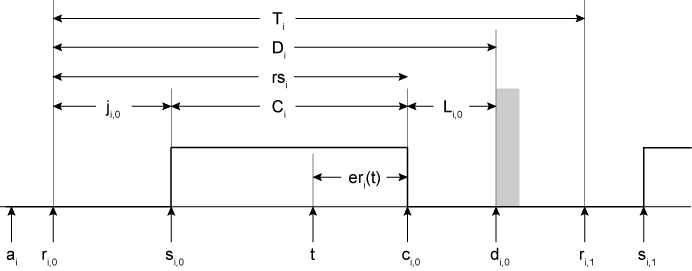
\includegraphics[width=0.7\textwidth]{master-exam-2014/figure1}
 
\item In the rate monotonic algorithm, the task with the ........... gets the highest static priority. ( Please fill in the blank )

\item In the earliest deadline algorithm, the task with the ............... gets the highest dynamic priority. ( Please fill in the blank )

\end{unteraufgaben}

\pagebreak

\aufgabe{}{10}


14.	The rate monotonic algorithm is a static priority scheduling algorithm and the earliest deadline first is a dynamic priority scheduling algorithm. Using T1 = ( 1, 4 ); T2 = ( 2, 6 ); T3 = ( 3, 8 ); where the value in parantheses are ( C, T ). Please assume the deadline to be the same as the period.

\begin{unteraufgaben}

\item	Calculate the processor utilization factor of the tasks for both the alorithms. Does the calculated factor suffice the schedulability test? Please answer why?
\item	Compute the hyperperiod of the tasks. 
\item	Fill in the chart to draw the schedulability of the tasks for both the algorithm.

\end{unteraufgaben}

\aufgabe{}{5}


Using T1 = ( 1, 4 ); T2 = ( 2, 8 ); T3 = ( 3, 12 ); where the value in parantheses are ( C, T ), please 

\begin{unteraufgaben}

\item	Calculate the processor utilization factor of the task using RM algorithm.
\item	Compute the hyperperiod of the task set. 
\item	Fill in the chart to draw the schedulability of the tasks using the RM algorithm.
\item	Can an aperiodic task with the release time of 2, deadline of 20 and computation time of 3 fit in this algorithm? Please calculate the response time of this aperiodic task.

\end{unteraufgaben}


\pagebreak

\aufgabe{}{5}

In the below precedence tasks with 9 tasks, please fill in the chart in accordance to the priority.

\begin{unteraufgaben}

\item	For a three processor system.
\item	For a four processor system. 

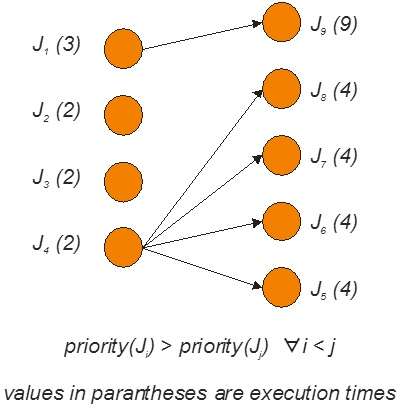
\includegraphics[width=0.5\textwidth]{master-exam-2014/figure2.jpg}

\end{unteraufgaben}

